\chapter{Introduction}

\begin{figure}
	\centering
	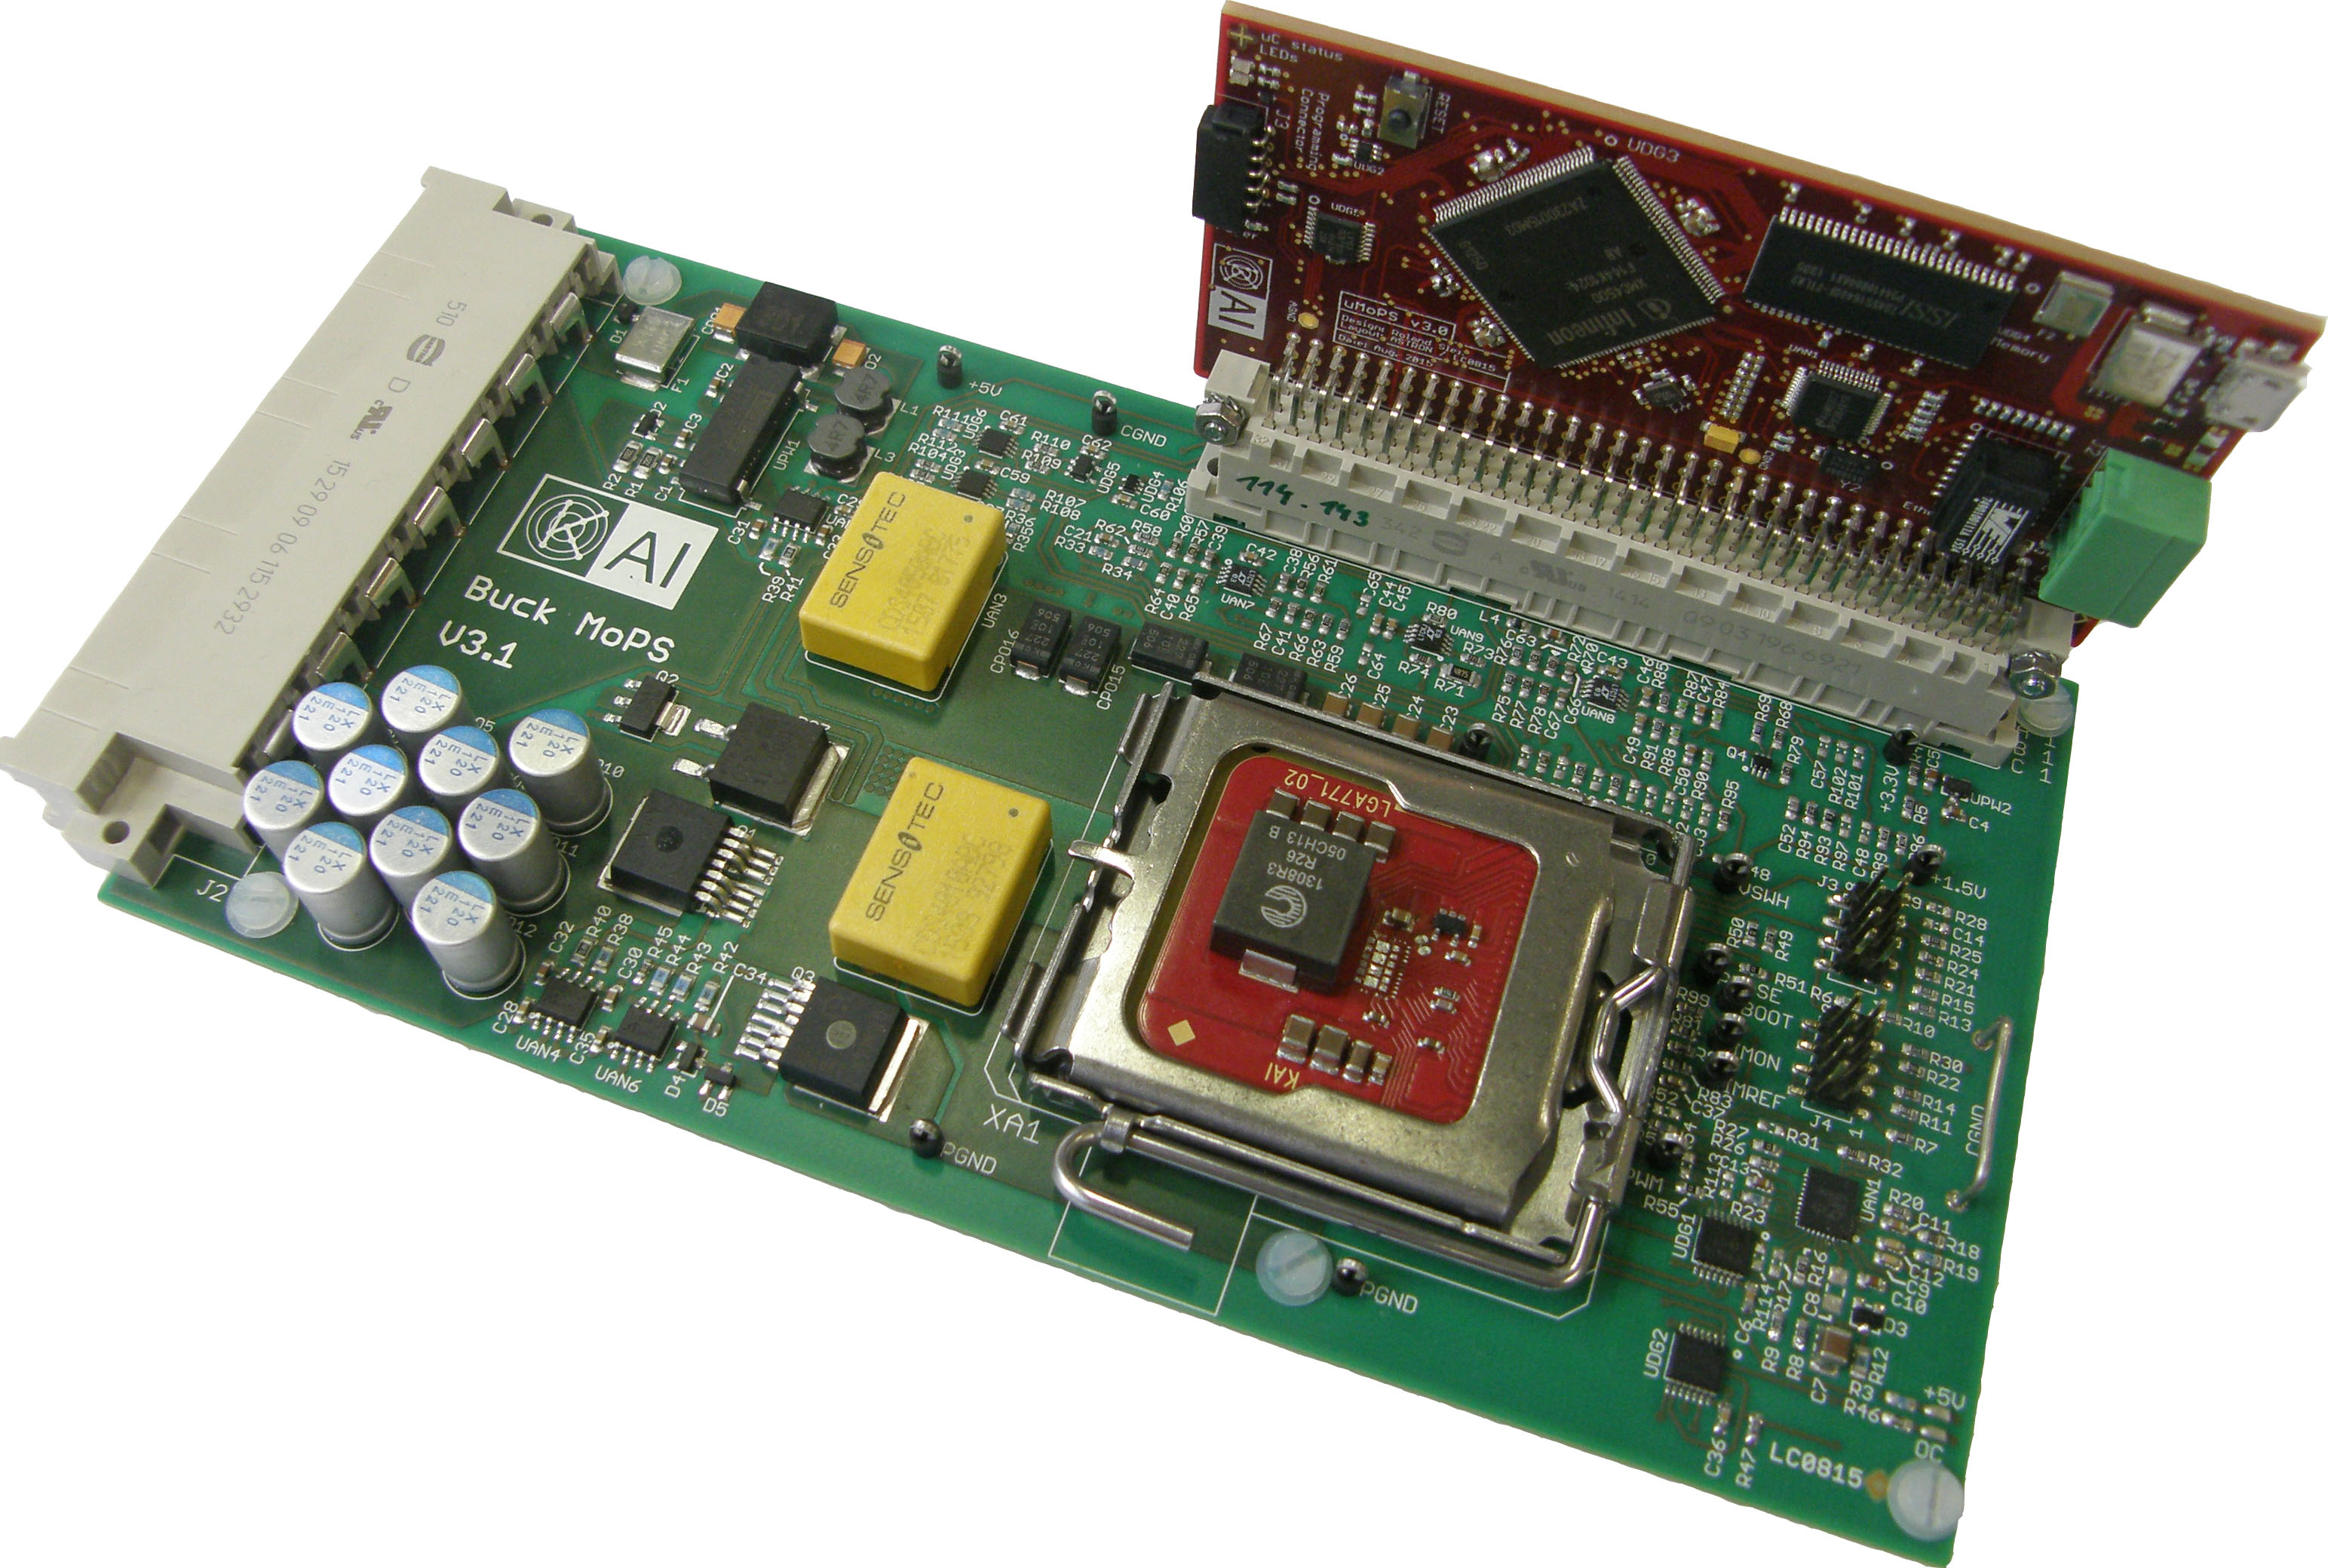
\includegraphics[trim=0 0 0 0, clip, width=100mm, scale=0.75]{images/Buck_and_uMoPS_2.jpg}
	\caption{MicroMoPS, BuckMoPS and LGA771 arrangement.}
	\label{fig:combination}
\end{figure}

\glspl{SoC} play a prominent role in the leap forward of today's technological evolution.
The ability to perform complex functionalities within a small object created the demand for the extensive need of \glspl{SoC} in almost every semiconductor industry.
\glspl{SoC} are leading to provide smart solutions for the dominant, real-life complex problems because of their intelligent features.
To utilize the benefits of the capabilities of \gls{SoC} and to ensure the operation of such micro computing environments and power devices, it is essential to predict the life span of the \gls{SoC} or \gls{DUT} that helps in determining the reliability to use the \gls{DUT} in the real world embedded applications. 
The determination of reliability of \gls{DUT} involves a classical procedure of introducing the semiconductor into various stress scenarios.
From the obtained behavior to predict the \glspl{SoC}' lasting capabilities and reliability.
This is a very essential procedure for semiconductor manufacturers during the development and release of any new semiconductor products. 
Various types of stress tests~\cite{Sleik2016} are performed to extract the characteristics of the \gls{DUT}. 
These stress tests obey a flexible test approach called the Modular test system.
This test system is split into two instances, namely the host system and the hardware module. 
The hardware module is termed as MicroMoPS in this test environment.
The host system is named as \gls{SAM} and controls the overall test flow and communicates with the MicroMoPS\footnote{MoPS stands for Modular Power Stress}.
Many MicroMoPS units may be connected to the host computer via an Ethernet network.
The host computer forwards the stress pattern to the MicroMoPS and receives preprocessed (digitized and filtered) measurement data application and status information.
The inclusion of the application module between MicroMoPS and the stress subjected semiconductor device is for integrating the test circuit, to monitor vital parameters of \gls{DUT} during test runs as well as to provide protection circuits to avoid catastrophic destruction of the test setup in case of a \gls{DUT} failure.
Each application module is connected to one MicroMoPS, which controls the application test, performs measurement data acquisition and logs device status information. 
The application modules are tailored to an individual type of test.
In this work, scaling functions such as Reverse Polish Notation (RPN) and linear scaling are incorporated into the data processing module of MicroMoPS for time and memory-efficient processing of analog measurements. Measurement circuits are analyzed to deduce the linear scaling equation that fits for the data processing system of the Modular test system. Also, the processing of data is automated via \gls{SAM} regardless of the type of stress test application that is performed. The attainment of high speed processing of analog measurements and the automation of processing of data are investigated on a particular stress test type called a Low Voltage stress test system. 
The application module and \gls{DUT} that are associated (\cref{fig:combination}) to the Low Voltage stress test system are termed as BuckMoPS and LGA771 respectively.  
    
\section{Problem Statement and Motivation}

\begin{figure}[htb]
	\centering
	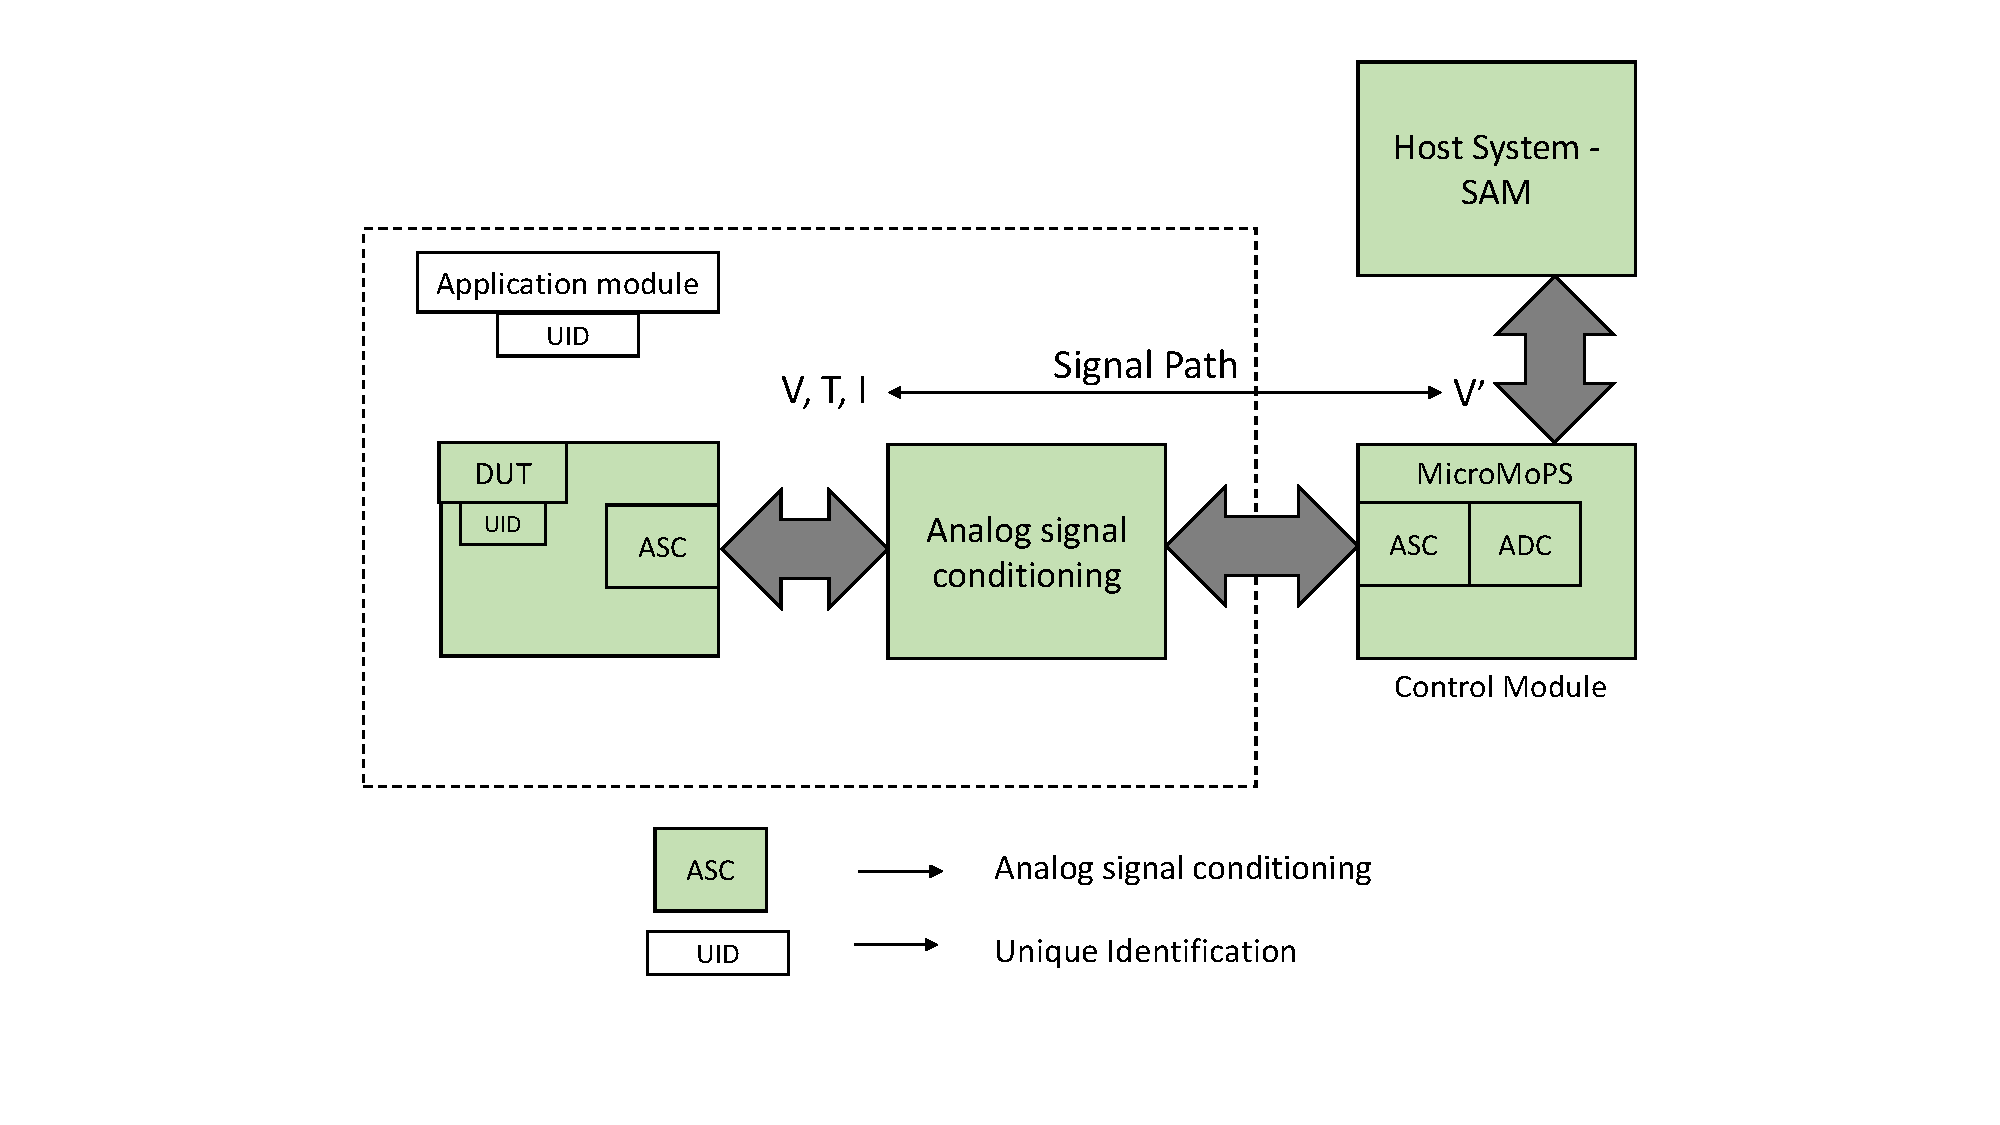
\includegraphics[trim=145 50 0 25, clip, width=\textwidth]{images/High-level signal conditioning.pdf}
	\caption{Measurement environment.}
	\label{fig:Signalmodelmotivation}
\end{figure} 

In this sophisticated test environment, the stress exertion on to the \gls{DUT} is achieved by running so-called \emph{test plans} in MicroMoPS. 
This test plan\cite{Plankensteiner2015} is created by test engineers.
When creating a test plan, it is necessary to initialize all the hardware parameters and test parameters. 
Also, the calculation of measurement related scaling parameters is described in the test plan. 
This method of manual scaling is error-prone and the scaling values may vary based on the type of stress test that is performed. 
Semiconductor devices are subjected to various application specific stress tests~\cite{Sleik2016} such as \emph{power cycling, automotive repetitive short circuit testing, and inductive clamping}. 
In order to avoid manual scaling, the procedure of scaling needs to be automated. 
This way, writing the test plan is simplified and human error possibilities are much reduced.
Using the \gls{SAM}~\cite{Steinwender2016} and the \gls{UID} of application module and \gls{DUT} module, the possibility of automation of data processing is identified.
Another concern is that, the data processing system of MicroMoPS uses a standard scaling mechanism to process the analog measurements~\cite{Sleik2016} into MicroMoPS operating voltage values.
But, from the analog signal conditioning circuit (see \cref{fig:Conditioning}) that lies between the source of the analog to digital converter of control module and source of the analog signal at the application module, there is a scope of deriving a linear scaling equation that processes the digital data in the control module. Introducing linear scaling over standard scaling function improves the speed of processing of analog measurements that are generated on \gls{SoC}.
Also, in a few other scenarios, the scaling function need not have to be linear because of the complex analog signal conditioning circuit that could exist in the measurement environment. To address this scenario, a memory-efficient mathematical notation called \acrshort{RPN} is introduced to the data processing system of the control module.
Hence, the linear scaling mechanism and \acrshort{RPN} mechanism are investigated for scaling in this work.
%Linear scaling equation is a very simple operation compared to RPN, which opens possibility for much more real-time efficient performance in measurement data acquisition.}
 

\section{Research Questions}\label{sec:RQs}
\begin{itemize}
	\item Is it possible to incorporate a robust scaling function to boost the performance of measurement data processing?
	\item Is it possible to derive a linear scaling equation in the test environment that involves complex measurement circuits?
	\item Is it possible to automate the method of scaling in the test environment?
\end{itemize}

\newpage
\section{Thesis Structure}

The rest of the thesis is structured as follows:

\begin{enumerate}
    \item \textbf{Chapter 2} provides a brief overview of the software tools, programming languages, and hardware peripherals that are used in this work.   
    \item \textbf{Chapter 3} presents the underlying concepts of the Modular stress test environment, hardware and software modules in the test environment, measurement data acquisition and processing concepts of MicroMoPS. 
    \item \textbf{Chapter 4} explores the milestones of this project, analysis of the measurement circuit and the approach at which the milestones are achieved.
    \item \textbf{Chapter 5} explains the performed software implementations concerning to the mentioned milestones. 
    \item \textbf{Chapter 6} describes the results that are obtained from performing this work and some analysis with the existing systems.  
    \item \textbf{Chapter 7} concludes the research work of this thesis and provides some recommendations for future works.
\end{enumerate}
